In this chapter, the origin of blockchain, its concepts, terms, related technique will be introduced, which lays the foundation of the whole master thesis. It starts from Bitcoin, where the blockchain technology was originated. Then followed by the process of its development and derivatives.

\section{Bitcoin}
Digital currencies (e.g. Flooz, Beenz) appeared with the tech tide in the 90s, which would have made the online payment and transaction more convenient,
however, most of those systems utilized a trusted third party (TTP) approach, meaning that the two-party trusted company verified and facilitated the transactions. On the one hand, this method will inevitable encounter single-failure problem, on the other hand, usual framework of digital currency made from digital signature may cause the double-spending problem. 

\textbf{Double-spending} \\
This problem is a potential flaw in a cryptocurrency or other digital cash scheme whereby the same single digital token can be spent more than once, and this is possible because a digital token consists of a digital file that can be duplicated or falsified.
\cite{DoubleSpend} 
\begin{figure}[H]% order of placement preference: here, top, bottom
	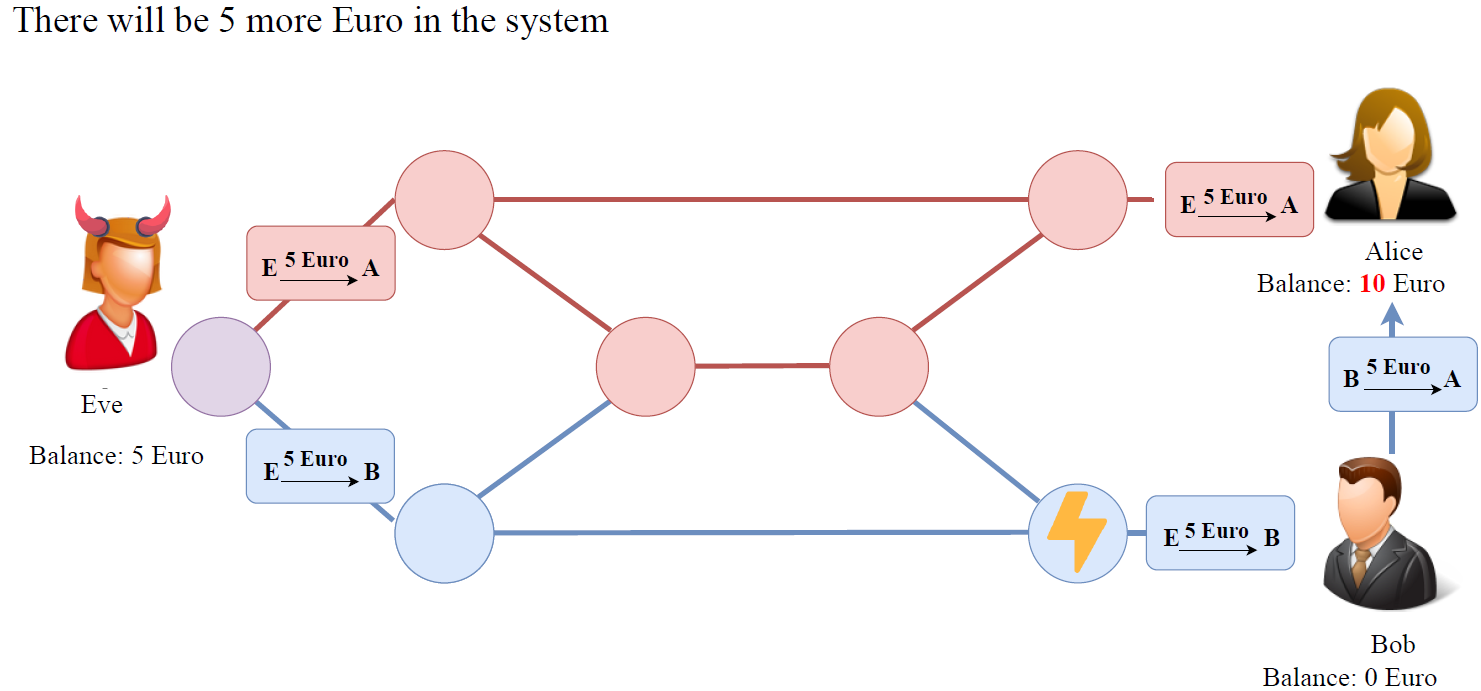
\includegraphics[width=\textwidth]{charts/DoubleSpend}
	\caption{Alice and Bob received repeated transaction }
\end{figure}

In 2008, a paper "Bitcoin: A Peer-to-Peer Electronic Cash System", written by Satoshi Nakamoto appeared on a US mailing list. This is the very beginning of Bitcoin. It proposed a mechanism based on the peer-to-peer network, using proof-of-work to record the public history of a transaction
that quickly becomes computationally impractical for an attacker to change if honest nodes control a majority of CPU power.

The network timestamps transactions by hashing them into an ongoing chain of hash-based proof-of-work, forming a record that cannot be changed without redoing the proof-of-work.\cite{sn} Bitcoin brought together a set of  techniques to enable the distrusting entities to transact directly with a digital currency. The following several elements are very important to help build Bitcoin system.

\subsection{Peer-to-peer network}

 In a general client-server network, a server takes charge of preservation and operation of data while clients request the server for the access of data and resource. On the contrary, in a P2P network, all participating nodes (referring to computers, also called "peers") hold data respectively and create an autonomous network wherein data are requested, meaning that each node acts both of server and client. P2P nodes have significant or total autonomy from central servers.

P2P networking technology has contributed to developing a base for a complete distributed network and eliminating single point of failure in Bitcoin.

\subsection{Cryptographic hash function}
A Cryptographic hash function is any function that can be used to map data of arbitrary size to data of a fixed size. This mechanism is characterized by the fact that the same hash value is obtained from the same data but only a slight difference in the original data results in a completely different hash value.

It is extremely difficult to infer the original data based on a hash value (non-invertible feature). Taking advantage of such characteristics, this mechanism is used for the detection of falsification of data, and in the Bitcoin system, it is used for the verification and guarantee the continuity of blockchain data and the creation of blockchain through Proof of Work utilizing the calculation of hash value.

\subsection{Consensus Mechanism}
The distributed nature of the peer-to-peer network requires the members (nodes) in the network to reach a consensus which validates the new coming data blocks which contain transactions by following a set of rules. The rules are specified in the algorithmic design of the blockchain system and can vary depending on its nature, purpose, and underlying asset.

In Bitcoin system, participants begin to propose the transactions. Before a transaction is allowed to be added to the global ledgers, other participants (also called miners) in the network first verify the validation of the transaction by solving a computational problem, once it is solved, they propagate answers to other miners along with the block of transactions. The other miners will accept the solutions along with the block of transactions and add those transactions to the global ledger. The Bitcoin transaction process is explained in the Figure 2.2.

The Bitcoin system, uses "Proof of work" (PoW) algorithm to establish consensus. Other frequently are used algorithms like Proof of Stake(PoS),  Practical Byzantine Fault Tolerance (PBFT).

\begin{figure}[!htb]% order of placement preference: here, top, bottom
	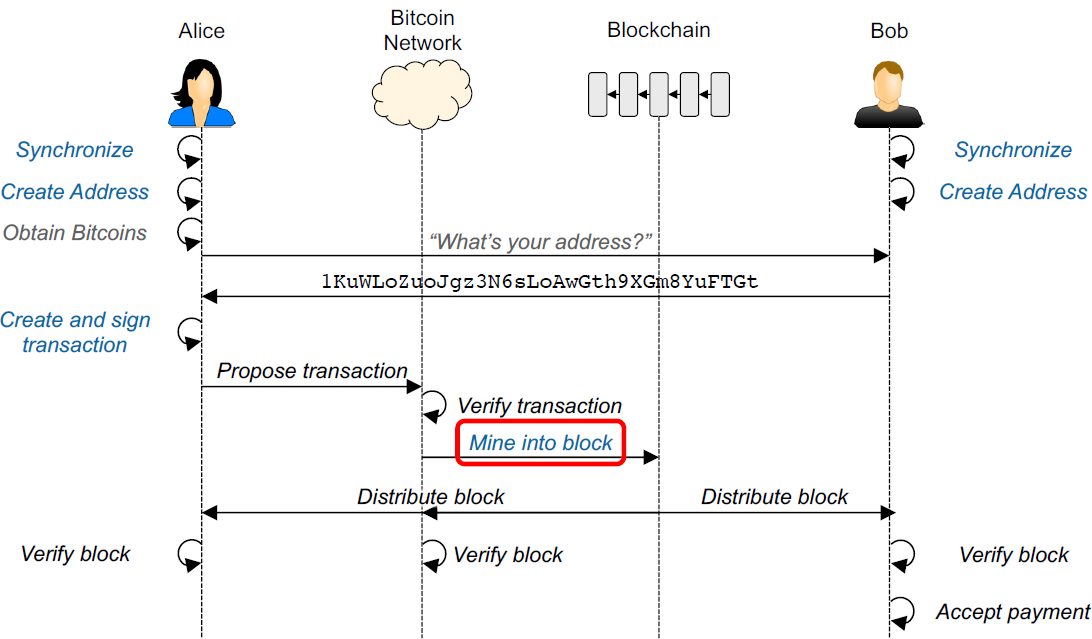
\includegraphics[width=\textwidth]{charts/BitcoinTx}
	\caption{Overview: Path of a Bitcoin Transaction\cite{sn}}
\end{figure}

\begin{itemize}
	\item \textbf{Proof-of-Work}
	
	Proof-of-Work (PoW) generally refers to a mechanism to confirm a node’s request for add a block (a block might contain several transactions) to the blockchain that involves solving a computational challenging puzzle in order to create a new block. PoW is also called mining in Bitcoin.
	
	\item \textbf{Proof-of-Stake}
	
	The Proof of Stake (PoS) algorithm is an energy-saving generalization of the Proof of Work algorithm. In PoS, the nodes are known as the "validators" and, rather than mining the blockchain they validate the transactions to earn a transaction fee. It based on the idea that the more stake of a node has, the more capable it can mine a block successfully. Thus nodes are randomly selected to validate blocks, and the probability of this random selection depends on the amount of stake held.
	
	\item \textbf{ Practical Byzantine Fault Tolerance (PBFT)}
	
	PBFT is an algorithm for solving a \textbf{Byzantine Fault} resulting from a failure in building a consensus caused by the Byzantine Generals Problem. Simply speaking, this algorithm ensures the consistency of consensus as long as two thirds of the network’s nodes are safe (i.e., not malicious or faulty). This is enabled by replicating behaviors (i.e., state machines) of generating nodes and applying protocols for choosing a leader among them. However,
	this method requires that all the generating nodes know each
	other since they need to communicate. In other words, all the
	parties have to agree on the exact list of participants.
	\cite{pbft}
	
	\item \textbf{Tendermint \cite{tendermint}}
	
    Tendermint is another byzantine consensus algorithm without mining work. It makes the assumption that the network is partially synchronized since the time factor is central to this protocol. For each new block, a validator node is selected in a round-robbin manner which has to propose a block. This block is then spread into the
    network and has to gather more than two thirds of votes of
    members within a given time period before being added to
    the blockchain. However, these members are selected based
    on their stake and thus ties trust to resource ownership.
\end{itemize}

\begin{table}[H] \centering 
%	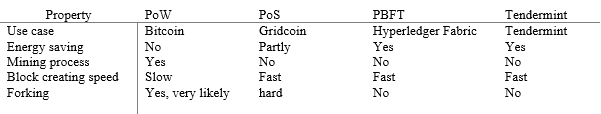
\includegraphics[scale=0.9]{charts/consensus}
     \ra{1.3}
     \begin{tabular}{{m}{3cm}ccccc}\toprule[0.5mm]
      Property & PoW & PoS & PBFT & Tendermint\\ 
      \midrule[0.3mm]
      Use case & Bitcoin & Gridcoin & Hyperledger Fabric& Tendermint\\
      Energy saving & No&Partly&Yes&Yes\\
      Mining process & Yes & No & No & No\\
      Block creating speed& Slow&Fast&Fast&Fast\\
      Forking& Yes, very likely&hard&No&No\\ 
      
      \bottomrule[0.5mm]
     \end{tabular}

	\caption{Typical Consensus Algorithms Comparison}
\end{table}
In the PoW the mining process is a brute-force approach, thus that is rather energy-consuming. While other algorithms without the mining process will be much more efficient. It also reflects on the speed of generating blocks. In the PoW, forking can happen if two miners find a suitable nonce at the same time. Meanwhile with
PoS, it is very difficult, happening only when a miner can own up to 51\% of all stake in the whole
verifying network. In the BFT-like consensus, e.g. PBFT and Tendermint, the validation essentially bases on the voting, it hardly forks.


\section{Blockchain Technology}
Blockchain originally came from Bitcoin's basic technology, referring a series of blocks created through PoW, and those blocks compiling transaction data for a certain period of time are linked into a chain. With the generalization of blockchain technology, it has more wide definition. Blockchain is a particular type of data structure used in some distributed ledgers which stores and transmits data in packages called "blocks" that are connected to each other in a "chain". Blockchain employs cryptographic and algorithmic methods to
record and synchronize data across a network in an immutable manner. \cite{WBank}

\begin{figure}[!htb]% order of placement preference: here, top, bottom
	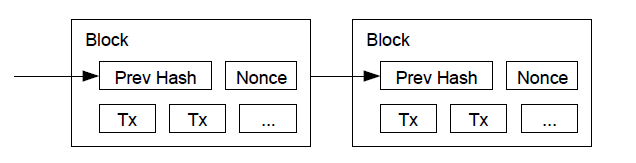
\includegraphics[width=\textwidth]{charts/blocks}
	\caption{blockchain appeared in Satoshi Nakamoto's paper}
\end{figure}

\subsection{Distributed Ledger Technology(DLT)}
Whenever the term blockchain is talked, frequently the related key word DTL would be mentioned.
Distributed Ledger Technology actually exists prior to Bitcoin, at least those techniques it represents are quite mature then. DLT is actually an umbrella term to the technology which is simply a decentralized database that is managed by various participants. Bitcoin blockchain is a milestone, which indicates the convergence of a host of technologies, including timestamping of transactions, Peer-to-Peer networks, cryptography, and shared computational power, along with a new consensus algorithm.

Distributed Ledger Technology generally consists of three basic components\cite{sawtooth}
\begin{description}
	\item [$\bullet$ A data model]that captures the current state of the ledger
	\item [$\bullet$ A transactions flow] that changes the ledger state
	\item [$\bullet$ A protocol] used to build consensus among participants around which transactions will be accepted, and in what order, by the ledger.
\end{description}
\textbf{Blockchain}, a particular
type of DLT, uses cryptographic and algorithmic methods to create and verify a continuously growing, append-only data structure that takes the form of a chain of so
called 'transaction blocks' – the blockchain – which serves the function of a ledger.\cite{WBank}

\subsection{Components of Blockchain system}
Having the foundation of Bitcoin's concept and DLT's structure, if we want to build a blockchain system, those components are likely required.

\begin{outline}
	\1 \textbf{Peer-to-peer network architecture}\\
	Due to the distributed nature, that each node in the network should keep a copy of the ledger. p2p network is the essential innovation shift to decentralized system.
	
    \1 \textbf{Consensus mechanism}\\
	As mentioned above, how consensus mechanism impacts the success of a blockchain system. It helps to validate the transaction, without the trusted third party.
	\1 \textbf{Smart contract}\\
	Smart contracts are simply predefined computer programs that execute actions when pre-agreed conditions within the system are met. Smart contracts provide the language of transactions that allow the ledger state to be modified. They can facilitate the business logic (e.g.  the exchange of shares, money, content, property). Smart contracts can be done in traditional centralized ledger systems as well, but the design of centralized ledger systems require such actions to be implemented only after the concerned parties have agreed to the underlying transaction as recorded in the central system.
		\2 \textbf{Decentralized Autonomous Organization(DAO)}\\
		A DAO can be seen as the most complex form of a smart contract, where the bylaws of the decentralized organization are embedded into the code of the smart contract, using complex token governance rules. At today’s evolutionary stage, a DAO materializes as a smart contract – a piece of code – executed on top of an increasingly opaque stack of distributed networking and consensus technology like the Ethereum blockchain or similar blockchains.\cite{dao}
	
	\1 \textbf{Cryptography}\\
	Cryptography has a key role to play both in the security, as well as in the immutability of the transactions recorded on blockchain . Cryptography is the study of the techniques used to allow secure communication between different parties and to ensure the authenticity and immutability of the data being communicated. For blockchain technology, cryptography is used to prove that a transaction was created by the right person. It is also used to link transactions into a block in a tamper-proof way, as well as create the links between blocks, to form a blockchain.
	
	
\end{outline}

\subsection{Types of Blockchain System}
Blockchain systems can be categorized as permissionless and permissioned. \textbf{Permissioned blockchain system} means that the parties that join the network are authenticated and authorized by an entity or
an administrator of the ledgers to participate on the network. while in \textbf{permissionless blockchain systems}, there is no central owner who controls network access. All that is needed to join the network and add transactions to the ledger is a server with the software.
The detailed comparisons are in the following Figure 2.4.\\
\begin{figure}[!htb]% order of placement preference: here, top, bottom
	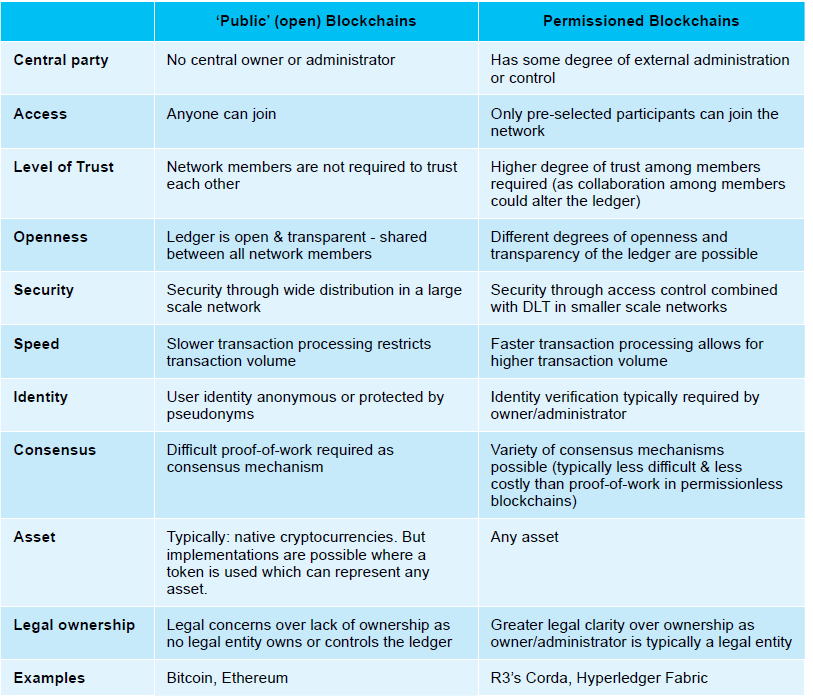
\includegraphics[width=\textwidth]{charts/permission}
	\caption{Comparison of permissioned and permissionless DLT}
\end{figure}
In permissionless blockchain systems, like the Bitcoin or the Ethereum, anyone can join the network, as well as write and read transactions. The actors in the system are not known, which means there could be some malicious actors within the network. Permissioned blockchain reduces these security risks and ensures that only the parties with valid identification can transact. 

There are several examples which base on the essential blockchain concepts and establish customized blockchain systems, which provide developers and companies with the architecture, where they can develop their own Dapps (Decentralized Applications).
  
\begin{itemize}
	\item \textbf{Ethereum} is an open blockchain platform(permissionless) that lets anyone build and use decentralized applications that run on blockchain technology.\cite{EthereumWhitePaper}  As the most popular blockchain for smart contracts, it facilitates the scripting functionality, or smart contracts which are run through the nodes in the network.
	\item  \textbf{Hyperledger Fabric} is a permissioned blockchain framework and one of the Hyperledger projects hosted by The Linux Foundation. Intended to create enterprise grade, open source, distributed framework for developing applications or solutions with a modular architecture. 
	\item  \textbf{Corda} is permissioned platform developed by R3 in collaboration with over 200 technology and industry partners. Smart contracts allow Corda to do this using complex agreements and any asset type. This capability has broad applications across industries including finance, supply chain and healthcare. 
	\item \textbf{IOTA} refers not only a cryptocurrency, but also a platform that entails a generalization of the blockchain protocol (the technology called Tangle) that sits at the backend of the IOTA platform. It enables machine-to-machine (M2M) transactions, which enhances the use of connected devices or the Internet of Things.
\end{itemize}

\subsection{Application of Blockchain Technology}
Deriving from Bitcoin, blockchain technology has a breadth of potential applications beyond cryptocurrencies in the financial field and in a wide variety of other industries.

According to World Bank's white paper, The two biggest trends in the development of blockchain applications are: 1) commercial Fintech start-ups are developing digital applications for a variety of purposes that utilize the public blockchain infrastructure, mostly Bitcoin and Ethereum;  2) industry consortia are forming to research and develop private, permissioned blockchain to solve industry-specific enterprise solutions. Actually the blockchain technology has been widely tried, in 2016 Nomura Research Institute have alreday conduct a survey on Blockchain Technologies, it visualized those applications based on Blockchain.
\begin{figure}[!htb]% order of placement preference: here, top, bottom
	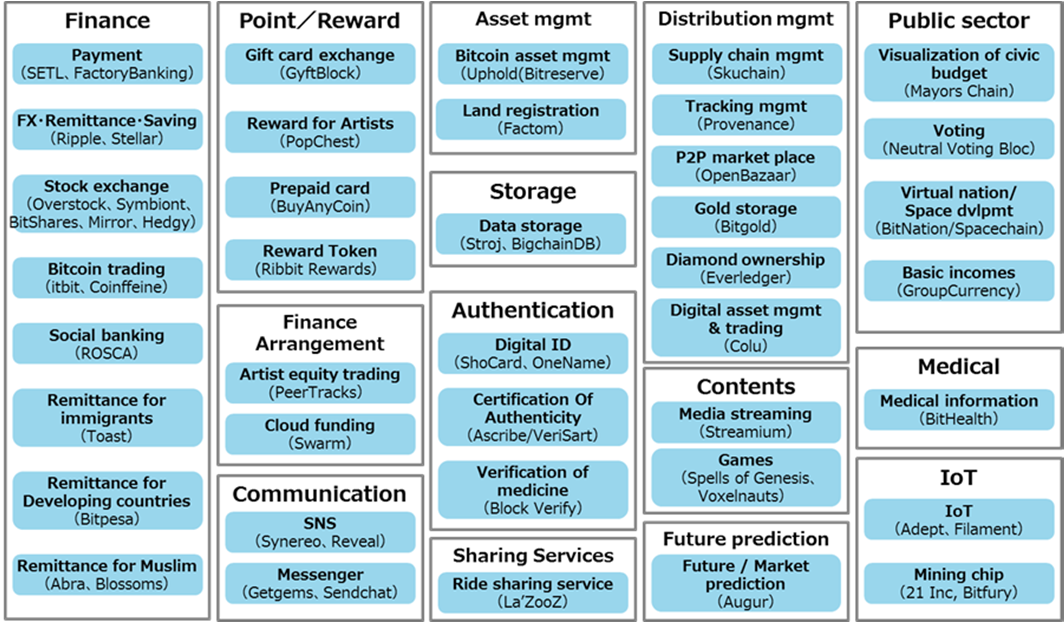
\includegraphics[width=\textwidth]{charts/Fields}
	\caption{Use cases and exmaples of services using blockchains\cite{JapanS}}
\end{figure}

\begin{itemize}
	\item \textbf{Finance}\\
	Ripple is one of the representative blockchains in this field.
	\item \textbf{Loyalty points and reward}\\
	GyftBlock, which provides an exchange service of gift
	cards using a blockchain.
	\item \textbf{Funding}\\
	Swarm provides a service to procure funds through cloud funding on a
	blockchain.
	\item \textbf{Communication}\\
	Messaging services and social networking services (SNS) have been
	made available using blockchains.
	\item \textbf{Asset management}\\
	Factom, etc. commenced the provision of a service.
	\item \textbf{Storage}
	Storj provides a service to manage various electronic files using a blockchain. Similar application like BigchainDB.
	\item \textbf{Authentication}\\
	uPort is a self-sovereign identity and user-centric data platform. 
	\item \textbf{Sharing}\\
	LaZooZ aims to provide a sharing service using a blockchain. At present, it provides a ride sharing application like Uber.
	\item \textbf{Commercial distribution management:}\\
	Everledger provides a system to manage
	diamonds. The serial number and carat, various commodity information, ownership and distribution record of each diamond are managed.
	\item \textbf{Content}\\
	Streamium provides a service to support content delivery, having established a system to charge by the second (paid with bitcoins) for video delivery, etc.
	\item \textbf{Prediction}\\
	Augur provides a decentralized prediction market platform where participants cast votes on various events to predict the future through the wisdom of the crowd.
	\item \textbf{Public}\\
	Neutral Voting Bloc (NVB) is a service provided in Australia, advocating itself as a new political party.
	\item \textbf{Medical services}\\
		BitHealth aims to achieve its goal to enable users to safely check
	their own health records from anywhere in the world using a blockchain.
	\item \textbf{IoT}\\
	Such services as ADEPT by IBM and Samsung are attracting attention.
	
\end{itemize}

